\documentclass[
  12pt,
  openright,
  twoside,
  a4paper,
  english,
  brazil
]{abntex2}

% Configurações de pacotes utilizados

\usepackage{lmodern}
\usepackage[T1]{fontenc}
\usepackage[utf8]{inputenc}
\usepackage{lastpage}
\usepackage{indentfirst}
\usepackage{color}
\usepackage{graphicx}
\usepackage{adjustbox}
\usepackage{microtype}
\usepackage[brazilian, hyperpageref]{backref}
\usepackage[alf]{abntex2cite}
\renewcommand{\backrefpagesname}
\renewcommand{\backref}{}
\renewcommand*{\backrefalt}[4]{}

% Dados para capa e folha de rosto

\titulo{Desenvolvimento de Aplicações em Java e\\Conceitos de UI e UX}
\autor{Pedro Felipe Froes Silva}
\local{Belo Horizonte}
\data{2017}
\orientador{Kécia Aline Marques Ferreira}
\coorientador{Avenue Code Desenvolvimento e Comércio de Softwares Ltda}
\instituicao{
  Centro Federal de Educação Tecnológica de Minas Gerais
  \par
  Departamento de Computação
  \par
  Curso de Engenharia de Computação
}
\tipotrabalho{Relatório}
\preambulo{Relatório apresentado ao Curso de Engenharia de Computação do Centro Federal de Educação Tecnológica de Minas Gerais, como requisito parcial para a aprovação na disciplina Estágio Supervisionado.}

% Configurações do PDF gerado

\definecolor{blue}{RGB}{41,5,195}
\makeatletter
\hypersetup{
  pdftitle={\@title},
	pdfauthor={\@author},
  pdfsubject={\imprimirpreambulo},
  pdfcreator={LaTeX with abnTeX2},
	pdfkeywords={estágio supervisionado}{java}{ui}{ux},
	colorlinks=true,
  linkcolor=blue,
  citecolor=blue,
  filecolor=magenta,
  urlcolor=blue,
  bookmarksdepth=4
}
\makeatother
\setlength{\parindent}{1.3cm}
\setlength{\parskip}{0.2cm}
\interfootnotelinepenalty=10000

% Inclusão de seções do trabalho

\makeindex
\begin{document}
\frenchspacing
\imprimircapa
\imprimirfolhaderosto*

%\begin{fichacatalografica}
%\end{fichacatalografica}

%\begin{folhadeaprovacao}
%	\begin{center}
%		Espaço destinado à folha de aprovação
%	\end{center}
%\end{folhadeaprovacao}

%\begin{dedicatoria}
%	\vspace*{\fill}
%	\centering
%	\noindent
%	\textit{Dedicatória a ser escrita.} \vspace*{\fill}
%\end{dedicatoria}

%\begin{agradecimentos}
%	Agradecimentos a serem escritos.
%\end{agradecimentos}

%\setlength{\absparsep}{18pt}

\begin{resumo}
	Este trabalho descreve as atividades desenvolvidas durante o período de Estágio Supervisionado do aluno Pedro Felipe Froes do curso de Engenharia de Computação do CEFET-MG enquanto estagiário na empresa Avenue Code. Parte do programa de Jedi Internship da empresa é descrita, focando nas áreas de aprendizador Java e desenvolvimento de interface de usuários (UI). Ambas as áreas têm sua fundamentação teórica presente no Capítulo~\ref{cap:fundamentacao-teorica} deste trabalho, e o Capítulo~\ref{cap:atividades-desenvolvidas} descreve as atividades desenvolvidas em cada uma delas. Finalmente, o Capítulo~\ref{cap:conclusao} conclui o trabalho.
	
	\textbf{Palavras-chave}: Estágio supervisionado. Java. \textit{User interface}.
\end{resumo}

%\begin{resumo}[Abstract]
%	\begin{otherlanguage*}{english}
%    	Abstract to be written.
%		\textbf{Keywords}: keyword.
%	\end{otherlanguage*}
%\end{resumo}

\pdfbookmark[0]{\listfigurename}{lof}
\listoffigures*
\cleardoublepage

%\pdfbookmark[0]{\listtablename}{lot}
%\listoftables*
%\cleardoublepage

\begin{siglas}
	\item[API] Interface de programação de aplicações (\textit{application programming interface})
	\item[CSS] Folhas de estilo em cascata (\textit{cascading stylesheets})
	\item[DAO] Objeto de acesso a dados (\textit{data access object})
	\item[JDBC] Java Database Connectivity
	\item[HTML] Linguagem de marcação de hipertexto (\textit{hyper text markup language})
	\item[UI] Interfaces de usuário (\textit{user interfaces})
	\item[WORA] Escreva uma vez, rode em qualquer lugar (\textit{Write once, run anywhere})
\end{siglas}

\pdfbookmark[0]{\contentsname}{toc}
\tableofcontents*
%\cleardoublepage

\textual
\chapter{Introdução}
\label{cap:introducao}

O presente trabalho é um relatório da disciplina de Estágio Supervisionado pertencente ao curso de Engenharia de Computação do Centro Federal de Educação Tecnológica de Minas Gerais (CEFET-MG), realizado pelo discente Pedro Felipe Froes Silva na empresa Avenue Code Desenvolvimento e Comércio de Software Ltda. Este relatório reflete o período de Março a Maio de 2017 durante o estágio do aluno na empresa, contemplando parte do Programa de Estágio Jedi Internship.

O Programa de Estágio Jedi Internship da Avenue Code corresponde a uma rotação dos participantes por diferentes tecnologias presentes na área de Computação. Durante o período do programa, o estagiário passa por cinco áreas distintas, obtendo um aprendizado de linguagens de programação como (i) Java e (ii) Ruby, (iii) do \textit{framework} .NET, (iv) de conceitos de garantia de qualidade de software, e (v) de conceitos e \textit{frameworks} para o desenvolvimento de interfaces de usuário (\textit{user interface}, UI) e experiência de usuário (\textit{user experience}, UX). O estudante exercita o aprendizado de cada área por meio de projetos internos da empresa, e apresenta um \textit{workshop} com o conteúdo aprendido ao final de cada etapa.

O objetivo desse trabalho é relatar as experiências do discente nas áreas em que o mesmo participou durante o período do Estágio Supervisionado, que correspondem ao aprendizado de Java e de conceitos de UI e UX. O aprendizado em cada uma das áreas é apresentado por meio do processo de desenvolvimento de um migrador de banco de dados em Java e da construção de interfaces de usuário por meio de \textit{frameworks} de UI e ferramentas de UX.

O restante desse trabalho está organizado de forma que o Capítulo~\ref{cap:estagio-supervisionado} apresenta a empresa e o seu Programa de Estágio, enquanto o Capítulo~\ref{cap:fundamentacao-teorica} aponta conceitos básicos de Java e de UI e UX. O Capítulo~\ref{cap:atividades-desenvolvidas} detalha as atividades em cada uma das áreas, enquanto o Capítulo~\ref{cap:conclusao} conclui o trabalho.

\chapter{Estágio supervisionado}
\label{cap:estagio-supervisionado}

Neste capítulo, a empresa concedente Avenue Code e o Programa de Estágio Jedi Internship são apresentados. Tópicos envolvendo a história, especialidade e iniciativas da empresa, bem como a estrutura do programa de estágio são ilustrado nas seções a seguir.

\section{Sobre a empresa: Avenue Code}
\label{sec:sobre-a-empresa}

A Avenue Code Desenvolvimento e Comércio de Softwares Ltd é uma empresa consultora de softwares especializada no ramo de \textit{e-commerce} da indústria varejista. Fundada em 2008 pelo CEO Zeo Solomon na cidade de San Francisco (Califórnia, EUA), a Avenue Code atendia clientes americanos, abrindo seu primeiro escritório no Brasil somente um ano depois, na cidade de Belo Horizonte. Nos anos seguintes, a empresa expande e inaugura um escritório na cidade de São Paulo, além de adicionar Amir Razmara e Chase Hill ao time de CEOs. Em 2017, a Avenue Code é formada por mais de 230 consultores em sua equipe, além de inaugurar um quarto escritório, agora na cidade de Nova York~\cite{avenuecode-2017}.

A Avenue Code é especialista no desenvolvimento e utilização de diversos tipos de tecnologias da área de Computação, como aplicações Web e móveis, automação de infraestruturas, sistemas de \textit{backend}, implementações de plataformas, \textit{coaching} Agile e DevOps e integrações corporativas. A Metodologia Ágil, oriunda do Manifesto Ágil para o Desenvolvimento de Software~\cite{agile-2001}, é altamente aplicada na empresa, que busca maximizar sua eficiência através da utilização de princípios Agile no desenvolvimento de projetos~\cite{avenuecode-2017}.

Prezando tanto pela qualidade da tecnologia utilizada quanto pelo ambiente de trabalho dos consultores, a Avenue Code possui uma gama de empresas parceiras e de prêmios obtidos em sua história. Dentre as empresas de tecnologia parceiras da Avenue Code, figuram a Mulesoft~\footnote{MuleSoft: Integration platform for connecting SaaS and enterprise applications. Disponível em: \url{https://www.mulesoft.com/}}, SAP Hybris~\footnote{SAP Hybris: E-commerce solutions. Disponível em: \url{https://www.hybris.com/en/}}, CHEF~\footnote{Chef: automate IT infrastructure. Disponível em: \url{https://www.chef.io/chef/}}, Oracle~\footnote{Oracle: Integrated cloud applications and platform services. Disponível em: \url{https://www.oracle.com/}}, Amazon Web Services~\footnote{Amazon Web Services: Cloud computing services. Disponível em: \url{https://aws.amazon.com/}} e Adobe~\footnote{Adobe: Creative, marketing and document management solutions. Disponível em \url{www.adobe.com/}}. Já entre os prêmios conquistados pela empresa, estão o reconhecimento pelo LoveMondays~\footnote{Love Mondays: A empresa ideal, avaliada por profissionais como você. Disponível em: \url{https://www.lovemondays.com.br/}}, InfoMoney~\footnote{InfoMoney: Notícias, ações e muito mais sobre investimentos. Disponível em: \url{www.infomoney.com.br/}} e San Francisco Business Times's Fast 100~\footnote{San Francisco Business Time Fast 100. Disponível em: \url{http://www.bizjournals.com/sanfrancisco/blog/2016/10/bay-area-fast-growing-private-companies-fast-100.html}} em 2016, além de ser agraciada como uma das Melhores Empresas para Trabalhar~\footnote{Great Place to Work. Disponível em: \url{www.greatplacetowork.com.br/}} em 2016 (\textit{Great Place to Work})~\cite{avenuecode-2017}.

Por fim, a Avenue Code participa de iniciativas de inclusão digital por meio do programa AC Social, que oferta aulas de introdução à tecnologias e computação em escolas carentes. A empresa também oferece cursos ministrados pelos próprios consultores por meio do AC Community, além de ofertar dois programas de estágios distintos, o AC Wonder Women e o Jedi Internship, que será apresentado na seção seguinte~\cite{avenuecode-2017}.

\section{Sobre o estágio: Programa de Estágio Jedi Internship}
\label{sec:sobre-o-estagio}

O Programa de Estágio Jedi Internship consiste de uma rotação (\textit{job rotation}) por cinco áreas de diferentes tecnologias presentes na área de Computação. São elas:

\begin{itemize}
	\item Conceitos e \textit{frameworks} de \textit{user interface} (UI) e \textit{user experience} (UX)
	\item Conceitos e \textit{frameworks} de garantia de qualidade de software
	\item Linguagem de programação Java
	\item Linguagem de programação Ruby
	\item \textit{Framework} .NET
\end{itemize}

Cada área dura cerca de três meses, e em cada uma delas o estagiário aprende conceitos introdutórios e avançados da tecnologia, aplicando-os em projetos internos da empresa. Cada área possui consultores que atuam como mentores para os participantes e, ao final da área, o estagiário elabora um \textit{workshop} para ser apresentado tanto para seus mentores quanto para os outros participantes do Programa, exibindo conceitos, aplicações desenvolvidas e desafios encontrados ao longo dos três meses.

Esse trabalho apresentará os conceitos aprendidos e aplicações desenvolvidas pelo autor ao longo das áreas de Java e UI/UX, sendo que uma fundamentação teórica para ambas as áreas é exibida no capítulo seguinte.
\chapter{Fundamentação teórica}
\label{cap:fundamentacao-teorica}

Neste capítulo, a fundamentação teórica das tecnologias abordadas neste trabalho é realizada. Conceitos básicos sobre a linguagem de programação Java são mostrados, abordando tanto os pilares da orientação a objetos presente na linguagem quanto bibliotecas relevantes para as aplicações desenvolvidas na área. Posteriormente, conceitos relevantes para a o desenvolvimento de interfaces de usuário (\textit{user interface}, UI) são apresentados, apontando características e ferramentas utilizada no processo de construção de interfaces.

\section{Java}
\label{sec:java}

Uma das tecnologias presentes no Programa de Estágio Jedi Internship e abordadas nesse trabalho corresponde ao aprendizado e aplicação de conceitos da linguagem de programação Java. Originada inicialmente em 1991 com o codinome de Oak, e nomeada de Java somente em 1995, atualmente a linguagem é uma das mais utilizadas na área de Computação, sendo administrada pela empresa Oracle e estando em sua oitava versão~\cite{ocastudyguide-2015}.

Em suas primeiras versões, o propósito inicial do Java era conectar diferentes tipos de micro-sistemas da empresa Sun, sendo uma linguagem comum entre eles. A habilidade de escrever um código que pode funcionar em mais de um sistema é conhecida como \textit{write once, run anywhere} (WORA), sendo uma das principais características da linguagem. Ao escrever um código em Java, o compilador Javac processa o arquivo fonte para um arquivo em \textit{bytecode}, e um interpretador JVM específico para a plataforma se encarrega de processar esse arquivo posteriormente, como mostrado na Figura~\ref{fig:java-fluxo}~\cite{ocastudyguide-2015}.

\begin{figure}[htb!]
  \centering
  \caption{Esquema de execução de um código escrito em Java.}
  \label{fig:java-fluxo}
  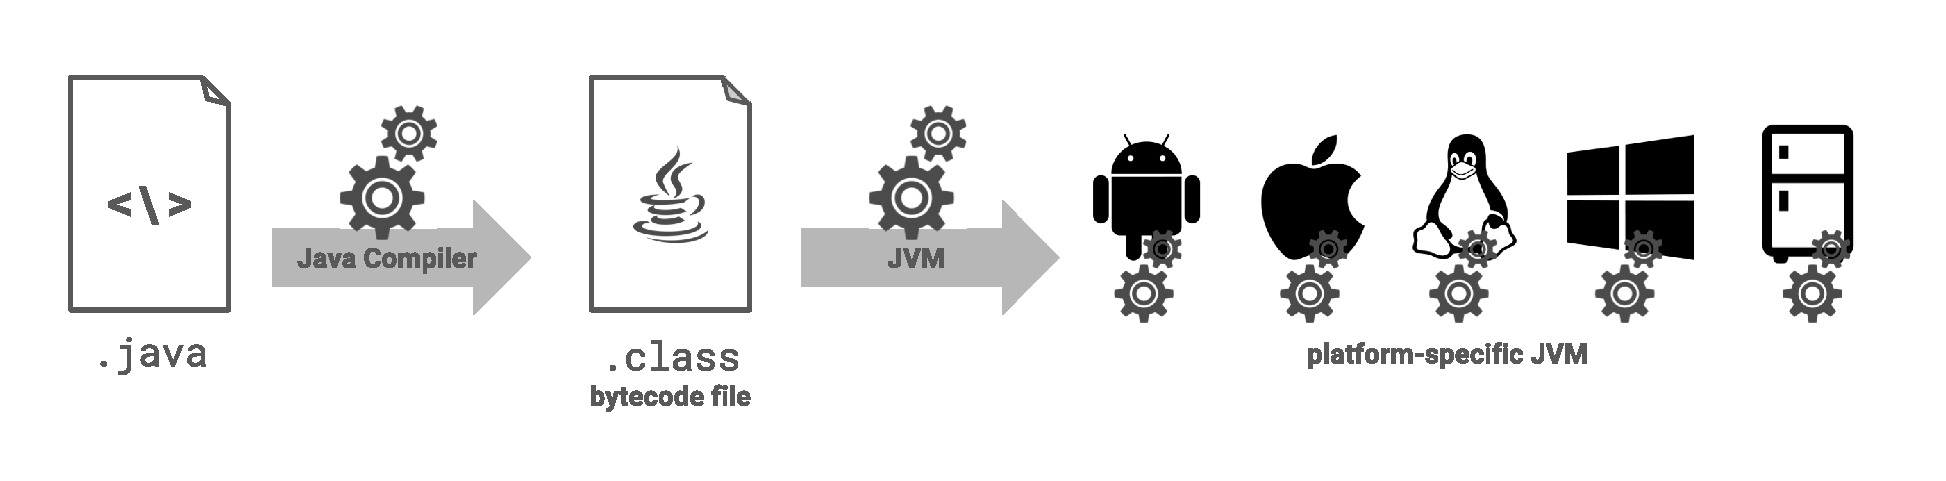
\includegraphics[width=\textwidth, keepaspectratio=true]{img/java-fluxo}
  \fonte{Próprio autor.}
\end{figure}

Além do WORA, outra característica marcante da linguagem é a implementação do conceito de orientação a objetos. Para implementar tal conceito, o Java faz uso de classes e objetos: enquanto uma classe funciona como uma especificação de uma ideia, um objeto corresponde a uma instância, uma materialização dessa ideia, sendo que uma classe pode possuir vários objetos instanciados~\cite{ocastudyguide-2015}.

A relação entre classes e objetos dá margem para diversos outros conceitos presentes na linguagem Java. O conceito de encapsulamento, por exemplo, faz uso de modificares de acesso nos atributos e métodos de cada classe para controlar quais objetos podem acessá-los, enquanto o conceito de herança entre as classes determina uma relação de pai-filho entre elas, tornando possível que uma herde atributos e métodos da outra~\cite{ocastudyguide-2015}.

Conceitos de abstração, composição e interfaces também estão presentes na linguagem, possibilitando a criação de classes não instanciáveis, classes compostas por diversos objetos, e a garantia que alguns métodos são implementados em determinadas classes, respectivamente. Por fim, um conceito essencial da linguagem é o polimorfismo, que permite que um objeto seja referenciado por diversas maneiras, como por meio das classes que ele herda, ou de interfaces que implementa~\cite{ocastudyguide-2015}.

Além dos conceitos apresentados, o Java ainda conta com bibliotecas como o \textit{collections framework}, que implementam diferentes estruturas de dados utilizadas comumente na programação de computadores. Estruturas como \textit{hashes}, listas de vetores, pilhas e filas podem ser utilizadas através das interfaces \verb|HashSet|, \verb|ArrayList|, \verb|Stack| e \verb|Queue|, respectivamente. Além de eliminar a necessidade do programador construir cada uma das estruturas, a utilização delas é extremamente comum em aplicações construídas em Java, facilitando o trabalho do desenvolvedor~\cite{javacollections-2001}.

Tanto os elementos presentes no \textit{collections framework} quanto os conceitos apresentados previamente podem ser utilizados para diversos tipos de aplicações em Java~\cite{javacollections-2001}. O gerenciamento de banco de dados relacionais em Java, por exemplo, utiliza uma interface de programação de aplicações (\textit{application programming interface}, API) chamada Java Database Connectivity (JDBC). O JDBC abstrai a implementação de banco de dados específicos, criando uma camada única que contribui para a implementação de métodos para estabelecer conexões, criar \textit{queries} de acesso, e extrair resultados de buscas, por exemplo~\cite{databaseprogramming-2000}.

O JDBC ainda conta com maneiras para gerenciar múltiplas conexões em um servidor através de um \textit{pool} de conexões, e de centralizar o acesso de dados por meio de objetos de acesso a dados (\textit{data access object}, DAO)~\cite{databaseprogramming-2000}. A utilização de alguns desses recursos é aprofundada na Seção~\ref{sec:java-atividades} do Capítulo~\ref{cap:atividades-desenvolvidas}, que descreve as atividades realizadas durante a área de Java do Programa de Estágio, focando na utilização da linguagem atrelada ao \textit{backend} de sistemas.

\section{Desenvolvimento de interfaces de usuário}
\label{sec:ui}

Uma das principais tarefas na construção do \textit{frontend} de um sistema é o desenvolvimento de interfaces de usuário (\textit{user interfaces}, UI). No desenvolvimento de uma aplicação Web, o designer de interfaces cria interfaces gráficas guiado por um designer de experiência de usuário (\textit{user experience}, UX), e passa as interfaces prontas para o desenvolvedor UI. Em posse das telas, cabe ao desenvolvedor transformá-las em código, o que ocorre essencialmente por meio da combinação de três tecnologias diferentes: a Linguagem de Marcação de Hipertexto (\textit{Hyper Text Markup Language}, HTML), as Folhas de Estilo em Cascata (\textit{Cascading Stylesheets}, CSS) e a linguagem de programação de propósito geral JavaScript~\cite{oppermann-2002, stefaner-2009}.

Para desenvolver as interfaces de usuário, é necessário primeiro construir a estrutura da página Web que irá abrigá-las, o que é feito por meio do HTML. O HTML dá estrutura para uma página Web, declarando formulários, \textit{links}, botões e outros elementos que possam estar presentes na interface por meio de \textit{tags}. Cada \textit{tag} pode ter uma gama de atributos – botões, por exemplo, podem ter alguma ação disparada quando são clicados por meio do atributo \verb|onClick|. Cada \textit{tag} é representada graficamente por diferentes \textit{browsers} de uma formas distintas, e utiliza-se então o CSS para dar um estilo próprio e único a cada um dos elementos~\cite{oppermann-2002, stefaner-2009}.

O CSS possibilita a estilização de diversas propriedades de cada elemento, como cores, tipografia, posicionamento e disposição na tela. Ainda é possível estilizar os elementos em diferentes estados que eles possam se encontrar, como quando o mouse os clica ou quando somente passa sobre eles. Além disso, é possível estilizar um grupo de elementos baseado em relações de hierarquia por meio de seletores CSS. Também é comum a utilização de pré-processadores de CSS como o SASS, que incluem a utilização de variáveis e uma sintaxe simplificada, por exemplo, para aumentar o desempenho e extender as funcionalidades do CSS~\cite{stefaner-2009}.

Por fim, o JavaScript é uma linguagem de programação de propósito geral que busca dar dinamismo para as páginas Web. Por meio dessa linguagem, é possível configurar as ações provenientes do disparo do botão mencionadas anteriormente, além de modificar o comportamento de elementos da página. Embora seja possível desenvolver interfaces de usuário somente por meio das três tecnologias, pode-se fazer uso de algum \textit{framework} JavaScript durante esse processo, como o AngularJS~\cite{angularjs-2017, oppermann-2002}.

O AngularJS é um \textit{framework} JavaScript que busca simplificar o desenvolvimento Web, possibilitando a utilização de uma arquitetura \textit{Model-View-Controller} (MVC) em uma aplicação Web. Criado por Hevery e Abrons em 2009, o \textit{framework} hoje encontra-se na versão 1.7, possuindo ainda uma versão 2 em fase de testes. Por meio do AngularJS, é possível conectar os dados exibidos na interface com um modelo constituído de variáveis e um controlador codificado em JavaScript que define métodos e lógica para a interface. A essa conexão dá-se o nome de \textit{data binding}, e uma das principais características do \textit{framework} em sua primeira versão é possibilitar o \textit{two-way data binding}, isso é, ocorre a conexão tanto do modelo com a interface quanto da interface com o modelo~\cite{angularjs-2017}.

Além do \textit{data binding}, o AngularJS também disponibiliza outras funcionalidades a fim de aumentar o dinamismo em aplicações Web, como diretivas, templates e filtros que podem ser incorporados diretamente no HTML por meio de atributos ou dentro de um arquivo JavaScript que contenha a lógica da interface~\cite{angularjs-2017}. Todas essas funcionalidades contribuem para o desenvolvimento de um projeto legível, com fácil manutenção e reutilização de código, sendo todas elas utilizadas nas atividades realizadas durante a área de UI do Programa de Estágio, mostrada na Seção~\ref{sec:ui-atividades} desse trabalho.
%\include{src/trabalhos-relacionados}
%\include{src/metodologia}
%\include{src/desenvolvimento}
\phantompart
\include{src/pos-textuais}
\end{document}
